\documentclass[12pt]{book}
\usepackage[utf8]{inputenc}
\usepackage[T1]{fontenc}
\usepackage{graphicx}
\usepackage{amsmath}
\usepackage{listings}
\usepackage{xcolor}
\usepackage{fancyhdr}
\usepackage{hyperref}
\usepackage{lipsum} % Only for generating text in this example

\hypersetup{
    colorlinks=true,
    linkcolor=blue,
    filecolor=magenta,      
    urlcolor=cyan,
}

% Configure header and footer
\pagestyle{fancy}
\fancyhf{} % Clear all header and footer fields
\fancyhead[LE,LO]{\slshape \leftmark} % Only chapter names in the left header
\renewcommand{\headrulewidth}{0.5pt}
\renewcommand{\footrulewidth}{0pt}

% Page style for the title page
\fancypagestyle{titlepagestyle}{
    \fancyhf{} % clear all header and footer fields
    \fancyfoot[R]{\textit{\small First Edition}} % Footer only on the title page
    \renewcommand{\headrulewidth}{0pt}
    \renewcommand{\footrulewidth}{0pt}
}

% Setting up the Python code style
\definecolor{codegreen}{rgb}{0,0.6,0}
\definecolor{codegray}{rgb}{0.5,0.5,0.5}
\definecolor{codepurple}{rgb}{0.58,0,0.82}
\definecolor{backcolour}{rgb}{0.95,0.95,0.92}

\lstdefinestyle{mystyle}{
    backgroundcolor=\color{backcolour},
    commentstyle=\color{codegreen},
    keywordstyle=\color{magenta},
    numberstyle=\tiny\color{codegray},
    stringstyle=\color{codepurple},
    basicstyle=\footnotesize\ttfamily,
    breakatwhitespace=false,
    breaklines=true,
    captionpos=b,
    keepspaces=true,
    numbers=left,
    numbersep=5pt,
    showspaces=false,
    showstringspaces=false,
    showtabs=false,
    tabsize=2
}

\lstset{style=mystyle}

\title{\textbf{A Text Book for Deep Learning in Hydrology}\\ \large For Hydrologists and Environmental Scientists}
\author{Kumar Puran Tripathy \\ Ashok Kumar Mishra}
\date{\today}

% Document starts here
\begin{document}

\thispagestyle{titlepagestyle} % Apply the custom page style to the title page
\maketitle % Generates title page

\tableofcontents % Generates table of contents

% Custom command to start chapters on a new page with Arabic numerals
\mainmatter

% \chapter{Introduction to Python}
\section{Why Python for DL?}
Python is our language of choice for hydrology and water resources engineering, offering a blend of simplicity and powerful functionality. Its straightforward syntax is easy for beginners to grasp, which contributes to its popularity in scientific fields, including machine learning. One of Python's greatest strengths is its extensive array of libraries. Libraries like NumPy, Pandas, and Matplotlib simplify tasks related to data handling, analysis, and visualization, making them less daunting and more efficient. These tools are crucial for hydrologists dealing with large and complex datasets.

Moreover, Python is the preferred language for TensorFlow and Keras, two of the most prominent libraries for DL. Their integration allows for advanced computational models, essential for modern hydrological research and applications. The combination of Python with these libraries opens up a world of possibilities in predictive modeling and environmental data analysis. In the following sections, we'll cover the basics of Python and these powerful libraries. For those already familiar with Python, you might choose to skim or skip these sections and proceed to the next chapter, where we dive deeper into specific hydrological applications using Python.

\section{Getting Started with Python}
\subsection{Installing Python and Setting Up the Environment}
To begin your journey with Python, the first step is installing the Python interpreter. You can download the latest version of Python from the official website: python.org. The website provides installation packages for various operating systems, including Windows, macOS, and Linux. Follow the installation instructions specific to your operating system. During installation, ensure that you select the option to add Python to your system's PATH, which makes it accessible from the command line.

For a more visual and guided setup process, consider watching tutorial videos on YouTube. Many content creators provide step-by-step guides on installing Python and setting up the environment, catering to different operating systems. These videos can be particularly helpful if you're new to installing software or configuring development environments. Opting for a video tutorial is often the quickest way to ensure a smooth and correct setup, allowing you to start coding in Python without unnecessary delays.

\subsection{Python IDEs and Editors}
While Python code can be written in any text editor, using an Integrated Development Environment (IDE) can significantly enhance your coding experience. IDEs provide features like syntax highlighting, code completion, and debugging tools. Some popular Python IDEs include PyCharm and Visual Studio Code. However, for DL applications, especially in hydrology and water resources engineering, we recommend using Jupyter Notebooks.

\subsection{Jupyter Notebooks: The Preferred Environment for DL}
We recommend using Jupyter Notebooks for several reasons, especially for beginners and those working on DL projects:

Interactive Development: Jupyter Notebooks provide an interactive development environment, allowing you to write and execute code in chunks (cells).
Experimentation and Visualization: They are ideal for experimentation, data analysis, and visualization—all crucial in DL.
Documentation and Sharing: Notebooks facilitate documentation and sharing of code, results, and explanations, making them excellent for educational purposes and collaborative projects.
For a cloud-based solution, Google Colab stands out as an exceptional choice. It offers a comparable interactive experience without the need for installation and is accessible from any web browser. Notably, Colab facilitates free GPU access, a boon for executing complex DL models. Discover more about \href{https://colab.research.google.com}{Google Colab}.

Both platforms, Jupyter Notebooks and Google Colab, support easy sharing and collaboration, including direct integration with GitHub. This feature is invaluable for DL practitioners, educators, and students alike, democratizing access to advanced computational resources and fostering a collaborative learning environment. As you delve into this book, utilizing Jupyter Notebooks will enrich your understanding of DL's practical applications in hydrology and water resources engineering, enhancing both learning and discovery.

\subsection{Writing Your First Python Program}
Once your Jupyter Notebook environment is set up, it's time to write your first Python program. Open Jupyter Notebook in your browser, create a new notebook, and you're ready to start coding. You can begin with a simple program, like printing a message:

\begin{lstlisting}[language=Python]
print("Welcome to DL in Hydrology")
output: [1] Welcome to DL in Hydrology
\end{lstlisting}

Type this into a Jupyter cell and execute it by pressing 'Shift + Enter'. Congratulations, you've just run your first Python program!

\section{Recommended Hardwares and GPU}

DL tasks in hydrology, such as predicting rainfall patterns, modeling watershed dynamics, or simulating flood events, require significant computational power. This section provides guidelines on the necessary hardware to efficiently run DL models, tailored for different levels of project complexity—from classroom projects to high-performance research applications.

\subsection{Basic Hardware for Classroom and Small Projects}
For individuals or students just starting with DL applications in hydrology:

\begin{itemize}
    \item \textbf{Processor (CPU)}: A modern multi-core processor (e.g., Intel i5 or i7, or AMD Ryzen 5 or 7) will be sufficient for basic data processing and smaller models.
    \item \textbf{Memory (RAM)}: At least 8GB of RAM, though 16GB is recommended for better multitasking and handling larger datasets.
    \item \textbf{Storage}: SSD storage of at least 256GB for faster data access and program loading times.
\end{itemize}

\subsection{Advanced Hardware for Research and Large Projects}
For researchers and larger projects that require more intensive computations and data handling:

\begin{itemize}
    \item \textbf{Graphics Processing Unit (GPU)}: A dedicated NVIDIA GPU is crucial for accelerating DL tasks. We recommend using at least an NVIDIA RTX 3060 for moderate projects. This GPU offers excellent performance for most DL tasks without breaking the budget.
    \item \textbf{High-Performance Computing (HPC) Configurations}:
    \begin{itemize}
        \item For advanced research requiring extensive simulations and model training, consider HPC resources equipped with NVIDIA Tesla or Quadro series GPUs.
        \item Multiple GPU setups can significantly reduce model training time. Systems such as NVIDIA DGX Stations or custom builds with multiple RTX 3090s are recommended for high-end computational needs.
    \end{itemize}
\end{itemize}

\subsection{Recommendations for High-Performance Computing}
For those with access to or considering investment in high-performance computing environments:

\begin{itemize}
    \item \textbf{Cluster Configuration}: A cluster with multiple NVIDIA A100 GPUs interconnected with high-speed networking (e.g., InfiniBand) ensures that large-scale models can be trained efficiently.
    \item \textbf{Memory and Storage}: High RAM capacity (256GB or more) and fast I/O storage solutions (NVMe SSDs in RAID configuration) are crucial for handling vast datasets and simultaneous processes.
\end{itemize}

\subsection{Additional Resources}
To further explore the specifications and capabilities of recommended GPUs and to stay updated with the latest advancements in computing hardware, please refer to the following resources:

\begin{itemize}
    \item \href{https://www.nvidia.com/en-us/deep-learning-ai/products/}{NVIDIA DL GPUs}
    \item \href{https://www.intel.com/content/www/us/en/high-performance-computing/hpc-overview.html}{Intel AI and HPC Solutions}
    \item \href{https://www.amd.com/en/processors/ryzen-for-business}{AMD Ryzen Processors}
\end{itemize}

By equipping yourself with the right hardware, you can ensure that your DL models operate efficiently, allowing you to focus more on innovation and less on computational limitations.

\section{Data Structures in Python}

\subsection{Lists and Tuples}
Python provides several compound data types, useful for grouping together other values. The most versatile of these are lists and tuples, which can be written as a list of comma-separated values between square brackets for lists, or parentheses for tuples.

\subsubsection{Creating Lists and Tuples}
\begin{lstlisting}[language=Python]
# Creating a list
rainfall = [20.5, 30.2, 25.4, 12.2]

# Creating a tuple
months = ('January', 'February', 'March', 'April')
\end{lstlisting}

\subsubsection{Accessing Elements, Slicing, and List Comprehensions}
\begin{lstlisting}[language=Python]
# Accessing elements
print(rainfall[1])  # Output: 30.2

# Slicing
print(months[0:2])  # Output: ('January', 'February')

# List comprehension
squared = [x**2 for x in range(5)]
print(squared)  # Output: [0, 1, 4, 9, 16]
\end{lstlisting}

\subsection{Dictionaries}
Dictionaries are another fundamental data structure in Python. They store mappings of unique keys to values and are incredibly efficient for retrieving data.

\subsubsection{Creating and Manipulating Dictionaries}
\begin{lstlisting}[language=Python]
# Creating a dictionary
river_flow = {'Amazon': 209000, 'Nile': 2830, 'Yangtze': 31900}

# Adding a new key-value pair
river_flow['Mississippi'] = 16200
\end{lstlisting}

\subsubsection{Importance of Dictionaries in Data Handling}
Dictionaries allow for rapid data retrieval via keys and are essential for data processing tasks where relationships between elements must be efficiently established and accessed.

\subsection{Sets and Frozensets}
Sets are collections of distinct (unique) items that are useful when you want to ensure no duplicates are present.

\subsubsection{Characteristics of Sets and Their Utility}
\begin{lstlisting}[language=Python]
# Creating a set
unique_rivers = set(['Amazon', 'Nile', 'Yangtze', 'Nile'])
print(unique_rivers)  # Output: {'Yangtze', 'Amazon', 'Nile'}

# Creating a frozenset
immutable_rivers = frozenset(['Amazon', 'Nile'])
\end{lstlisting}

Sets are particularly useful in data processing for operations like union, intersection, and difference, which can help in filtering and comparing datasets.

\section{Data Structures in Python}

Data structures are fundamental ways of organizing data to ensure efficient access and modification. Python simplifies learning these fundamentals compared to other programming languages, making it an ideal choice for hydrologists and environmental scientists.

\subsection{Lists}
Python lists are versatile and can be compared to arrays in other programming languages but with the added benefit of being able to store different types of data. Lists in Python are dynamic, meaning they can grow or shrink, and they are implemented similarly to vectors in C++ or ArrayLists in Java.

\subsubsection{Basic List Operations}
\begin{lstlisting}[language=Python]
# Creating a List with hydrological data points
rainfall_mm = [20, 30, 45, 50]
print("Monthly Rainfall in mm: ")
print(rainfall_mm)

# Creating a Multi-Dimensional List for different regions
region_rainfall = [['North', 20], ['South', 30]]
print("\nRegion-Wise Rainfall:")
print(region_rainfall) 

# Accessing elements using positive and negative indexing
print("\nAccessing the first and last element:")
print(rainfall_mm[0], rainfall_mm[-1])
\end{lstlisting}

\subsubsection{List Comprehension}
List comprehensions provide a concise way to create lists. Common applications include creating new lists where each element is the result of some operations applied to each member of another sequence or iterable.

\begin{lstlisting}[language=Python]
# Using list comprehension to square numbers
squared_numbers = [x**2 for x in range(6)]
print("\nSquared numbers from 0 to 5:")
print(squared_numbers)
\end{lstlisting}

\subsection{Dictionaries}
Dictionaries in Python are hash tables that store data in a key-value pair. They provide very fast O(1) time complexity for looking up data and are particularly useful in scenarios where the dataset is large and search speed is critical.

\subsubsection{Using Dictionaries in Hydrology}
\begin{lstlisting}[language=Python]
# Creating a dictionary to store river discharge rates
discharge = {'Amazon': 209000, 'Nile': 2830, 'Yangtze': 31900}
print("River discharge rates (cubic meters per second):")
print(discharge)

# Accessing data by river name
print("\nDischarge of the Nile:")
print(discharge['Nile'])

# Using get() to safely access elements
print("\nDischarge of the Ganges:")
print(discharge.get('Ganges', 'No data available'))
\end{lstlisting}

\subsubsection{Dictionary Comprehension}
Dictionary comprehensions offer a method to succinctly create dictionaries from a set of values.

\begin{lstlisting}[language=Python]
# Creating a dictionary to map river names to their lengths
river_length = {river: length for river, length in [('Amazon', 6400), ('Nile', 6650)]}
print("\nRiver lengths in kilometers:")
print(river_length)
\end{lstlisting}

\subsection{Tuples}
Tuples are immutable sequences in Python, used to store collections of heterogeneous data. Tuples are particularly useful when you need a fixed set of elements that should not change throughout the program.

\subsubsection{Creating and Using Tuples}
\begin{lstlisting}[language=Python]
# Defining a tuple for geographic coordinates
coordinates = (40.7128, -74.0060)
print("Coordinates of New York City:")
print(coordinates)

# Single element tuple, notice the comma
single_tuple = ('single',)
\end{lstlisting}

Tuples are not just immutable lists; they can be used as keys in dictionaries or as elements in sets, which is not possible with lists due to their mutability. This characteristic makes tuples incredibly useful in high-performance computing scenarios where data integrity and speed are paramount.

These sections provide a robust introduction to Python data structures with practical examples that demonstrate their application in environmental science and hydrology. This approach not only helps in understanding Python's capabilities but also illustrates its practical benefits in scientific computing.



\chapter{Fundamentals of Deep Learning}


\chapter{Fundamentals of Deep Learning}
% ---------------------------------------- Major Branches of Deep Learning -------------------------
\section{Major Branches of Deep Learning}
\subsection{Supervised Learning}
Supervised learning is one of the most widely used branches of deep learning. It involves training models on datasets where each input is paired with a corresponding output, commonly referred to as a \textit{label}. This approach enables models to learn the relationship between inputs and their known results, allowing them to make accurate predictions on new, unseen data. In essence, supervised learning is like teaching a system through examples where the correct answers are already provided.
Supervised learning tasks typically fall into two categories:
\begin{itemize}
\item \textit{Classification:} Sorting data into predefined categories. For example, classifying land cover types (e.g., forests, urban areas, water bodies) based on satellite images.
\item \textit{Regression:} Predicting continuous numerical values. An example is forecasting river water levels based on historical data and environmental conditions.
\end{itemize}
Supervised learning plays a pivotal role in hydrology and environmental sciences, powering a wide range of applications such as image classification, temperature forecasting, and hurricane tracking. To tackle these tasks, specific deep learning architectures are particularly effective. For example, Recurrent Neural Networks (RNNs) and their advanced variant, Long Short-Term Memory networks (LSTMs), excel at processing and forecasting sequential data, making them ideal for analyzing time-series datasets like rainfall records or river flow patterns. On the other hand, Convolutional Neural Networks (CNNs) are exceptionally adept at handling image-based tasks. They are commonly used for interpreting satellite images, such as identifying land cover types or detecting environmental changes.
Here are some representative examples of how supervised learning is applied in hydrology and environmental sciences:
\begin{itemize}
    \item \textit{Precipitation Forecasting:} Predicting rainfall amounts to aid in water resource management and flood prevention.
\item \textit{Drought Severity Classification:} Determining the severity of droughts to assist in agricultural planning and water conservation.
\item \textit{Land Cover Classification:} Categorizing earth surface types (e.g., forests, croplands, urban areas) from satellite imagery for applications like urban planning and ecosystem monitoring.
\item \textit{Image Segmentation:} Identifying specific regions in satellite images, such as flood-affected areas, deforested zones, or crop health conditions.
\item \textit{Object Detection:} Identifying and categorizing objects in satellite imagery, such as water bodies, vegetation types, or urban areas.
\end{itemize}


\subsection{Unsupervised Learning }

Unsupervised learning focuses on uncovering patterns, structures, and transformations within data, all without relying on labeled outputs. Instead of predicting a specific target, it aims to reveal insights such as correlations, clusters, or low-dimensional representations. This type of learning is invaluable in hydrology and environmental sciences, where complex datasets often need to be distilled into more interpretable or actionable forms. 
Unsupervised learning is foundational for tasks like data visualization, where the goal is to represent high-dimensional data in an intuitive way, and dimensionality reduction, which simplifies large datasets while retaining essential information. It also plays a critical role in data denoising, improving the quality of noisy remote sensing data to make subsequent analyses more reliable. Before solving supervised learning problems, unsupervised learning can act as a crucial first step to explore and understand the dataset, identify outliers, and discover hidden relationships.

\begin{itemize}
    \item \textit{Data Visualization:} Creating intuitive visual representations of high-dimensional datasets, such as water quality measurements spanning multiple variables, to better understand spatial and temporal trends.
    \item \textit{Dimensionality Reduction:} Simplifying vast climatic datasets, like global temperature records or precipitation grids, for faster processing and storage while preserving critical patterns.
    \item \textit{Data Denoising:} Enhancing the quality of noisy remote sensing data (e.g., satellite imagery or LiDAR scans) to improve the accuracy of downstream analyses like land cover classification or flood mapping.
    \item \textit{Clustering:} Identifying groups in the data, such as categorizing regions based on similar hydrological characteristics or climate patterns, without pre-defined labels.

\end{itemize}


\subsection{Self-Supervised Learning}

Self-supervised learning is a DL approach where the model generates its own labels directly from the input data, removing the need for human-annotated labels. These pseudo-labels guide the learning process, making it possible to utilize large amounts of unlabeled data. This is particularly beneficial in hydrology, where labeled datasets are often limited or incomplete.

A key advantage of self-supervised learning is its scalability. By automatically generating pseudo-labels, it avoids the time and cost associated with manual labeling. A well-known example of self-supervised learning is the autoencoder, a model that compresses data into a compact representation (the "encoder") and then reconstructs it back to its original form (the "decoder"). The reconstruction error—the difference between the input and the reconstructed output—provides the learning signal. We will explore autoencoders in detail in Chapter~\ref{chap:acn} with a practical example.

Here are two simple examples to illustrate self-supervised learning:

\begin{itemize}
    \item \textit{Noise Removal in Satellite Images:} Autoencoders can clean noisy satellite images by learning to reconstruct meaningful features, such as water boundaries, while removing noise.
    \item \textit{Predicting Missing Data:} Models can predict missing streamflow values based on surrounding data, helping to fill gaps in hydrological records for further analysis.
\end{itemize}

\textbf{NOTE:} In this book, we’ll primarily focus on supervised learning, as it remains the most widely used and impactful form of deep learning in hydrology and environmental sciences, powering applications like precipitation forecasting, flood mapping, and drought prediction. We’ll also briefly explore self-supervised learning in later chapters, as it offers promising solutions for leveraging large, unlabeled datasets, which are common in these fields.

\subsection{Reinforcement Learning}
There is another branch of DL called Reinforcement Learning (RL), where an agent interacts with its environment, learning through trial and error to take actions that maximize a reward signal. Unlike traditional DL, which focuses on mapping inputs to outputs, RL emphasizes decision-making in dynamic environments. For example, an RL model could determine optimal reservoir release strategies by balancing flood control and water conservation. While RL has shown success in fields like robotics and gaming, its applications in hydrology are still largely in the research phase. In this book, we will primarily focus on supervised learning, leaving RL for further exploration in advanced studies.

% ----------------------------------------Evaluating Deep Learning Models -------------------------






















\section{Evaluating Deep Learning Models}
Understanding how to evaluate deep learning models effectively is crucial for developing robust neural networks.

\subsection{Data Splits: Training, Validation, and Test Sets}
\begin{itemize}
    \item Discuss the importance of dividing the data into training, validation, and test datasets to prevent overfitting and estimate the model's performance on new data.
\end{itemize}

\subsection{K-fold Cross-Validation with Shuffling}
\begin{lstlisting}[language=Python]
# Example Python code for k-fold cross-validation with shuffling
from sklearn.model_selection import KFold
import numpy as np

data = np.array([...])  # Example data array
kfold = KFold(n_splits=5, shuffle=True, random_state=42)

for train, test in kfold.split(data):
    # Apply training and testing here
\end{lstlisting}

% --------------------------------- Data Processing and Feature Engineering ----------------------

\section{Data Processing and Feature Engineering}
\begin{itemize}
    \item \textbf{Normalization and Vectorization:} Techniques to scale and convert data into a format suitable for deep learning.
    \item \textbf{Handling Missing Values:} Strategies for dealing with incomplete datasets.
    \item \textbf{Feature Engineering:} Discuss how effective features can be engineered from data to improve model performance.
\end{itemize}
% --------------------------------- Overfitting, Underfitting, and Model Optimization ---------------

\section{Overfitting, Underfitting, and Model Optimization}
\begin{itemize}
    \item Discuss the signs of overfitting and underfitting and their implications on model performance.
    \item Explore strategies to achieve the optimal fit, including adjusting the model size.
\end{itemize}

\section{Techniques to Combat Overfitting}
\begin{itemize}
    \item \textbf{Weight Regularization:} Add L1 or L2 regularization to the model.
    \item \textbf{Dropout:} Randomly dropping units from the neural network during training to prevent over-reliance on any single neuron.
    \item \textbf{Batch Normalization:} Standardize the inputs to a layer within a mini-batch to stabilize the learning process.
\end{itemize}
% --------------------------------- Universal Workflow of Deep Learning ---------------

\section{Universal Workflow of Deep Learning}
Outline the standard steps involved in a deep learning project:
\begin{enumerate}
    \item Defining the problem and the data inputs.
    \item Choosing metrics and methods for evaluation.
    \item Engineering features from the data.
    \item Developing models to combat overfitting.
    \item Implementing interpretive mechanisms to understand model predictions.
\end{enumerate}

\section{Summary}
Summarize the key points discussed in the chapter and reiterate the importance of a systematic approach to developing deep learning models.


\section{Evaluating Deep Learning Models}
Understanding how to evaluate deep learning models effectively is crucial for developing robust neural networks.

\subsection{Data Splits: Training, Validation, and Test Sets}
To evaluate a model, we divide our dataset into three distinct sets:

\begin{enumerate}
    \item \textit{Training Set:} Used to train the model. The model learns patterns and adjusts its parameters on this data.
    \item \textit{Validation Set}: Used to tune the model’s hyperparameters, such as the number of layers or learning rate. It acts as a feedback mechanism to guide model improvements without being part of training.
    \item \textit{Test Set:} Used to assess the model’s final performance. It represents completely unseen data and ensures that the model generalizes well beyond the data it was trained or validated on.
\end{enumerate}

\paragraph{Why Not Just Use Two Sets? \newline}

At first glance, splitting the data into only training and test sets might seem simpler. However, developing a model often involves hyperparameter tuning, where decisions about the model’s architecture or training process are made based on its performance during development. Relying only on the test set for this tuning can lead to \textit{information leaks}, where the test data indirectly influences the model. This results in overly optimistic evaluations that don’t reflect real-world performance. The validation set prevents this by acting as an intermediate checkpoint. The test set is kept untouched until the very end, ensuring a fair assessment.

\paragraph{The Risk of Overfitting the Validation Set\newline}

Repeatedly tuning a model based on validation performance can inadvertently make the model overly specialized to the validation data. This happens because small amounts of information about the validation set "leak" into the model during each tuning step. If this process is repeated many times, the validation set’s reliability as an unbiased evaluation metric diminishes. To ensure a truly robust evaluation, the test set must remain untouched throughout the development process.


% --------------------------------- Overfitting, Underfitting, and Model Optimization ---------------

\section{Overfitting, Underfitting, and Model Optimization}
\label{sc:overfitting}
In the previous examples—temperature forecasting, classifying drought severity, and modeling lake water temperatures—we observed a common trend: the performance of the model on held-out validation data often peaked after a few training epochs and then began to degrade. This phenomenon, where a model performs well on training data but poorly on unseen data, is known as \textit{overfitting}. Overfitting is a challenge faced in every deep learning project, and mastering strategies to combat it is crucial for building effective models.
At the heart of this challenge is the tension between \textbf{optimization} and \textbf{generalization}:
Optimization refers to the process of training a model to perform as well as possible on the training data. Essentially, this is the \textit{learning} in DL. Generalization, on the other hand, is the ability of the trained model to perform well on unseen data.
Our ultimate goal is to achieve good generalization. However, generalization cannot be directly controlled during training; we can only adjust the model based on its performance on the training data. Understanding this balance is key to building robust models for hydrology and environmental sciences.
At the beginning of training, optimization and generalization are typically aligned: as the model's performance on the training data improves, so does its performance on validation data. During this stage, the model is said to be \textit{underfitting}. Underfitting occurs when the model has not yet captured all the relevant patterns in the training data, leaving room for improvement.

However, after a certain number of training iterations, a turning point is reached where the performance on the validation data stops improving. Beyond this point, continued optimization on the training data causes the model to overfit. \textit{Overfitting occurs when the model begins to memorize patterns that are specific to the training data} rather than learning generalizable patterns. These irrelevant patterns do not translate well to unseen data, leading to degraded performance on the validation set.

The most effective way to prevent overfitting is to \textit{increase the amount of training data}. With more diverse and representative data, the model can naturally generalize better to unseen examples. However, in many cases—especially in hydrology and environmental sciences—collecting additional data can be costly, time-consuming, or even impossible due to physical and logistical constraints.
When more data is not an option, the next-best approach is to restrict the amount of information the model can store or impose constraints on how it learns. This ensures the model focuses on the most relevant patterns in the data, which are more likely to generalize well. Techniques that achieve this are collectively referred to as \textbf{regularization}, which are discussed in section \ref{sc:reg}.


Regularization introduces constraints that limit a model's capacity to memorize irrelevant patterns, helping it generalize better. The underlying idea is simple: if a model can only "afford" to store a limited number of patterns, it will prioritize learning the most prominent and meaningful ones. Regularization methods include:


In the next section, we will explore these regularization techniques in detail and demonstrate how to apply them to improve the performance of a precipitation classification model.







\subsection{Weight Regularization}
\subsection{Early Stopping}
Early stopping is another effective technique for avoiding overfitting. It monitors the model’s performance on a validation set during training and stops training when performance on the validation set stops improving. This prevents the model from continuing to train and overfit the training data.

For example, a DL model might overfit after 100 epochs even though validation performance peaked at 50 epochs (\ref{fig:earlystop}). Early stopping stops the training process automatically, saving time and ensuring the best-performing model is retained.
In Keras, early stopping is implemented using the \textit{EarlyStopping} callback. For example:

\begin{lstlisting}[language=Python]
from keras.callbacks import EarlyStopping

# Define an EarlyStopping callback
early_stopping = EarlyStopping(monitor='val_loss', patience=5, restore_best_weights=True)

# Train the model 
model.fit(X_train, y_train, validation_data=(X_val, y_val), epochs=100, callbacks=[early_stopping])

\end{lstlisting}
Here:
\begin{itemize}
    \item \texttt{monitor= 'val\_loss'} tracks the validation loss.
    \item patience=5 means training stops if validation loss does not improve for 5 consecutive epochs.
    \item \texttt{restore\_best\_weights=True} ensures the best model is saved.
\end{itemize}

\subsection{Dropout Regularization}
Dropout is a simple yet powerful technique where a fraction of neurons in a layer is randomly "dropped out" during each training step. These dropped-out neurons do not contribute to the forward pass or the backward pass (gradient updates). This forces the network to learn more robust features by ensuring that no single neuron or group of neurons becomes overly specialized or reliant on specific connections.

For example, imagine a network that predicts runoff based on rainfall, temperature, and soil moisture. If some neurons are randomly deactivated during training, the network must learn alternative pathways and redundant features, improving its ability to generalize.

Key points about dropout:

\begin{itemize}
    \item Dropout is applied only during training, not during testing.
    \item The dropout rate specifies the fraction of neurons to drop (typically between 0.2 and 0.5).
    \item It works like training an ensemble of smaller subnetworks, which combine into a stronger overall model.
\end{itemize}
Adding dropout to a model in Keras is straightforward. For example:
\begin{lstlisting}[language=Python]
from keras.models import Sequential
from keras.layers import Dense, Dropout
# Define a model with dropout
model = Sequential([
    Dense(64, activation='relu', input_shape=(10,)),  # Input layer
    Dropout(0.3),  # Dropout layer with 30% rate
    Dense(32, activation='relu'),
    Dropout(0.2),  # Dropout layer with 20% rate
    Dense(1, activation='sigmoid')  # Output layer])
model.compile(optimizer='adam', loss='binary_crossentropy', metrics=['accuracy'])
\end{lstlisting}
\subsection{Batch Normalization}
\subsection{K-fold Cross-Validation}
K-fold cross-validation is a practical technique to evaluate model performance and reduce overfitting (discussed in detail in section \ref{sc:overfitting}), especially when data is limited. It works by dividing the dataset into k equal parts, called folds. For instance, if \textit{k=4}, the data is split into 4 subsets (Figure \ref{fig:kfold}). The model is trained on 3 folds and validated on the 1 remaining fold. This process is repeated 4 times, so each fold serves as the validation set exactly once. The final performance is averaged across all 4 runs, providing a robust estimate of the model's ability to generalize to new data.

This method ensures that all data points are used for both training and validation, making the most of limited datasets. For example, if the data is not shuffled before splitting, similar types of data (e.g., seasonal trends in hydrological data) might cluster in one fold, leading to biased results. By shuffling the data beforehand, each fold becomes more representative of the entire dataset, improving the reliability of the evaluation.

K-fold cross-validation is essential because it reduces the risk of overfitting. It ensures the model is tested on different subsets of data, exposing it to various patterns and reducing dependency on any single data split.



\begin{figure}[h!]
    \centering
    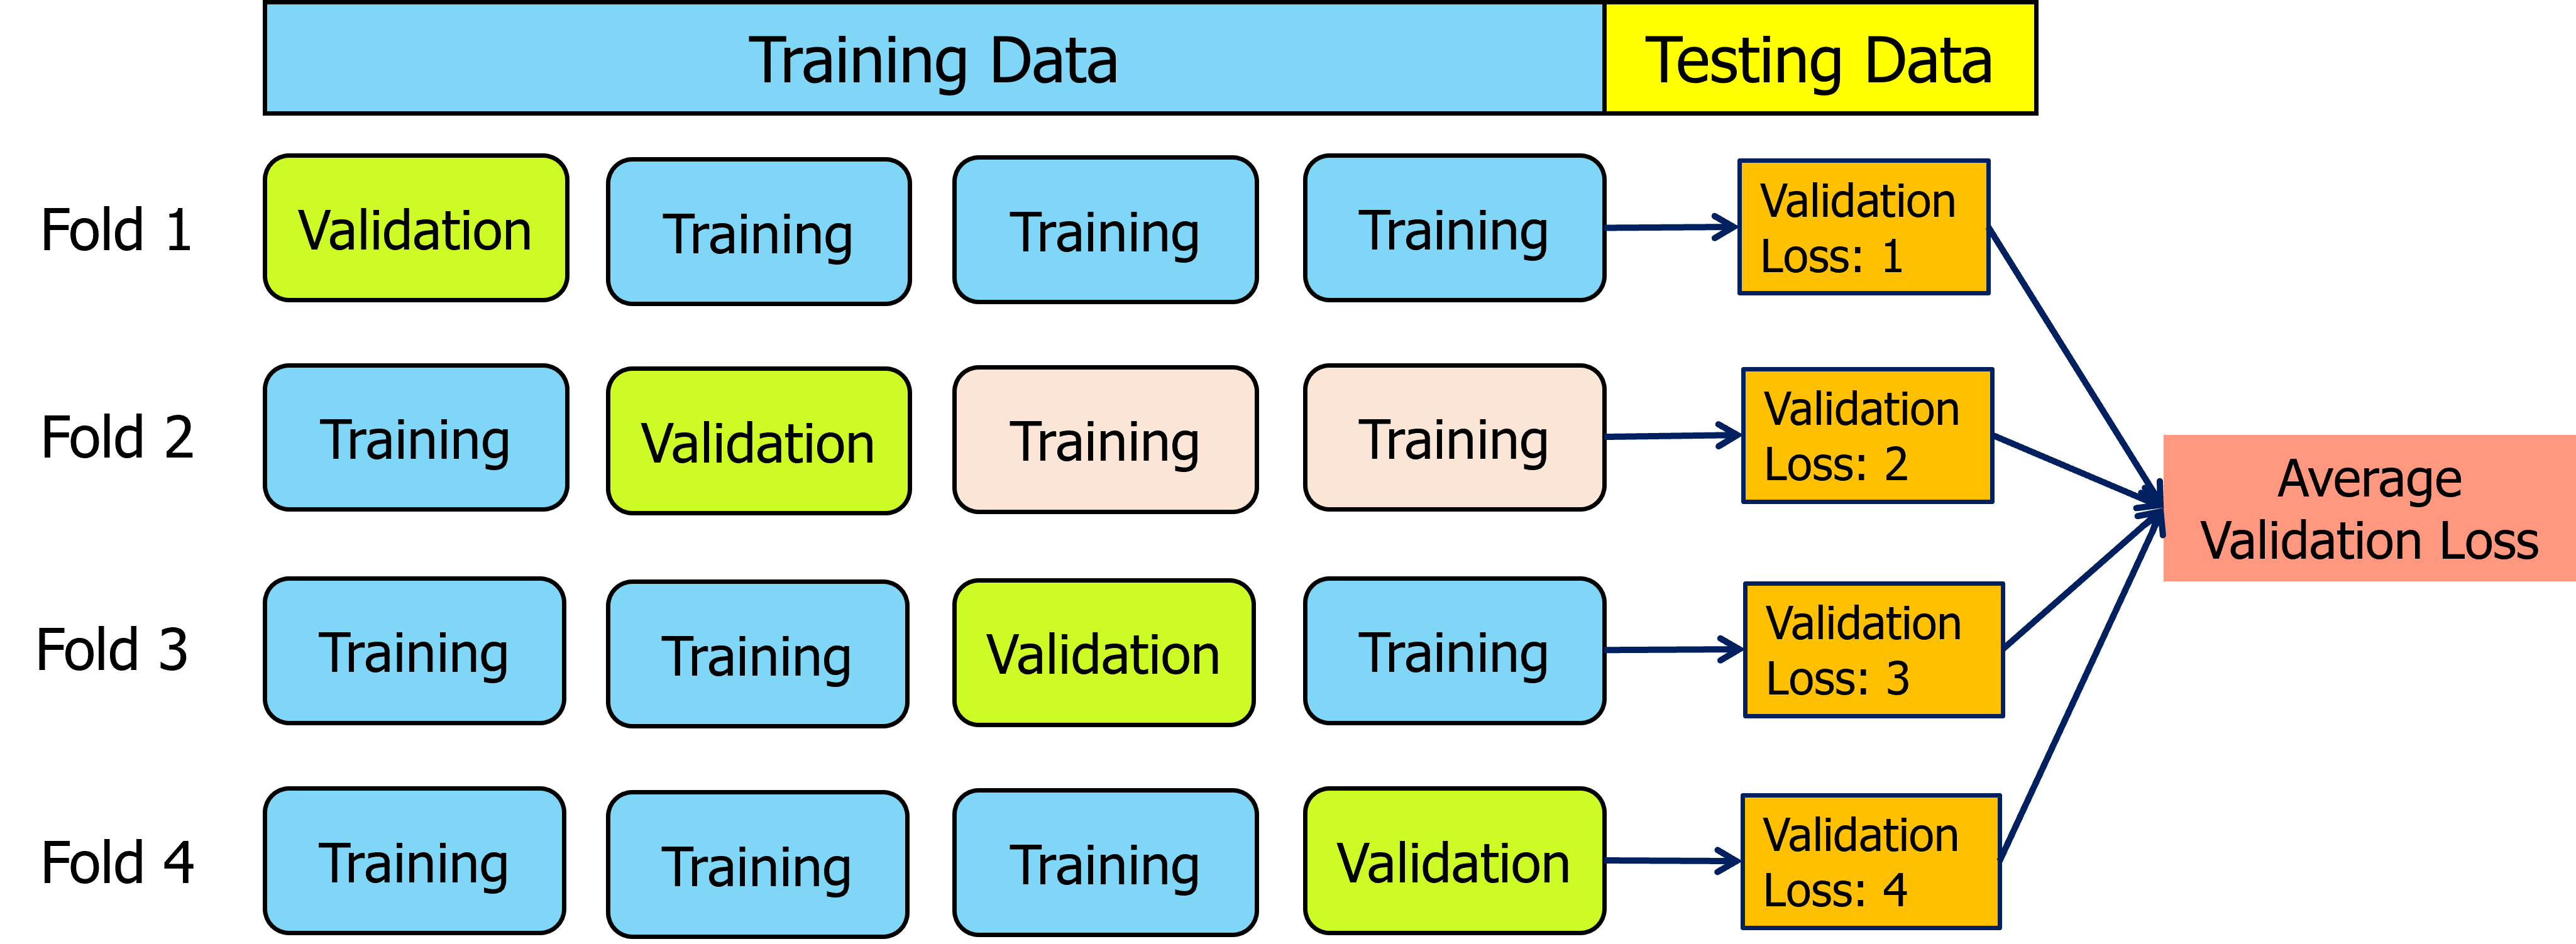
\includegraphics[width=\linewidth]{images/k-foldcrossval.png}
    \caption{K-fold Cross-Validation: The training data is divided into multiple subsets (folds). Each fold takes a turn as the validation set while the rest are used for training. The final validation score is the average of validation losses across all folds.}
    \label{fig:kfold}
\end{figure}


\begin{lstlisting}[language=Python]
# Example Python code for k-fold cross-validation with shuffling
from sklearn.model_selection import KFold
import numpy as np

data = np.array([...])  # Example data array
kfold = KFold(n_splits=5, shuffle=True, random_state=42)

for train, test in kfold.split(data):
    # Apply training and testing here
\end{lstlisting}
% --------------------------------- Data Processing and Feature Engineering ----------------------

\section{Data Processing and Feature Engineering}
\begin{itemize}
    \item \textbf{Normalization and Vectorization:} Techniques to scale and convert data into a format suitable for deep learning.
    \item \textbf{Handling Missing Values:} Strategies for dealing with incomplete datasets.
    \item \textbf{Feature Engineering:} Discuss how effective features can be engineered from data to improve model performance.
\end{itemize}

% --------------------------------- Universal Workflow of Deep Learning ---------------

\section{Universal Workflow of Deep Learning}
\label{sc: udl}
Outline the standard steps involved in a deep learning project:
\begin{enumerate}
    \item Defining the problem and the data inputs.
    \item Choosing metrics and methods for evaluation.
    \item Engineering features from the data.
    \item Developing models to combat overfitting.
    \item Implementing interpretive mechanisms to understand model predictions.
\end{enumerate}



% ------------------------------------ SUMMARY ----------------------------------------------
\section{Summary}
Summarize the key points discussed in the chapter and reiterate the importance of a systematic approach to developing deep learning models.




% \chapter{Autoencoders}
\label{chap:acn}


\include{chapters/machine_learning}
\include{chapters/deep_learning_applications}
\include{chapters/case_studies}

% Appendices and index would go here
\appendix
\include{chapters/appendix}

\end{document}
